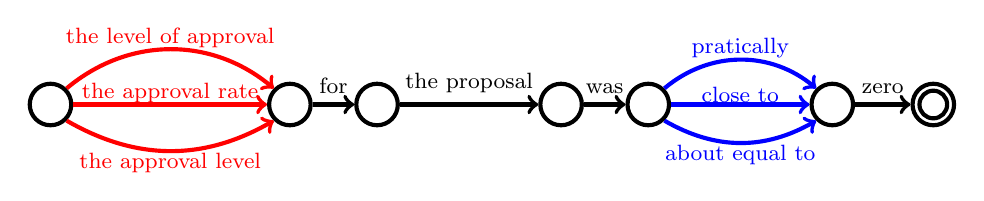
\begin{tikzpicture}	
	\tikzstyle{unit} = [circle,line width=1.5pt,draw,minimum size=1.5em]
		
		\node[unit] (u1)at (0,0){};
		\node[unit,anchor=west](u2) at ([xshift=7em]u1.east){};
		\node[unit,anchor=west](u3) at ([xshift=1.5em]u2.east){};
		\node[unit,anchor=west](u4) at ([xshift=5em]u3.east){};
		\node[unit,anchor=west](u5) at ([xshift=1.5em]u4.east){};
		\node[unit,anchor=west](u6) at ([xshift=5em]u5.east){};
		\node[unit,anchor=west,line width=1.5pt](u7) at ([xshift=2em]u6.east){};
		\node[unit,anchor=west,line width=1.5pt,minimum size=1em](u8) at ([xshift=2.25em]u6.east){};
		
		\draw[->,out=40,in=140,red,line width=1.5pt] (u1.north east) to  node[inner sep=0pt,color=red,above]{\footnotesize the level of approval}(u2.north west);
		\draw[->,red,line width=1.5pt](u1.east)-- node[inner sep=0pt,color=red,above]{\footnotesize the approval rate}(u2.west);
		\draw[->,out=-30,in=-150,red,line width=1.5pt] (u1.south east) to  node[inner sep=0pt,color=red,below]{\footnotesize the approval level}(u2.south west);
		\draw[->,line width=1.5pt](u2.east) -- node[above]{\footnotesize for} (u3.west);
		\draw[->,line width=1.5pt](u3.east) -- node[above]{\footnotesize the proposal} (u4.west);
		\draw[->,line width=1.5pt](u4.east) -- node[above]{\footnotesize was} (u5.west);
		\draw[->,out=40,in=140,blue,line width=1.5pt] (u5.north east) to  node[inner sep=0pt,color=blue,above]{\footnotesize pratically}(u6.north west);
		\draw[->,blue,line width=1.5pt](u5.east)-- node[inner sep=0pt,color=blue,above]{\footnotesize close to}(u6.west);
		\draw[->,out=-30,in=-150,blue,line width=1.5pt] (u5.south east) to  node[inner sep=0pt,color=blue,below]{\footnotesize about equal to}(u6.south west);
		\draw[->,line width=1.5pt](u6.east) -- node[above]{\footnotesize zero} (u7.west);
\end{tikzpicture}
